% TARI29_Assignment_report_template.tex
% This is a template for the assignment reports
% TARI29 Artificial Intelligence, 7.5 credits, Winter 2024
% Original version by:  Vladimir Tarasov, 2024
% Revised by:           Alexandros Tzanetos, 2024 

% Use a modern class instead of an old article class
\documentclass{scrartcl}

\KOMAoptions{
    parskip=half,  % full, off
    fontsize=12pt, % base font size (10pt default)
    % headings=big,% small/normal/big headings (normal is default), 
    % paper=a5,    % paper format (a4 default) 
    pagesize=auto  % Use paper format for PDF too
}

% ---------------------- Report details --------------------- %
%\newcommand{\docauthor}{Name1, Name2, Name3}
\newcommand{\courseyear}{2024}
\newcommand{\coursename}{TARI29 Artificial Intelligence}
\newcommand{\coursecredits}{7.5 credits}
\newcommand{\fullcoursename}{\coursename, \coursecredits}
\newcommand{\termname}{Winter \courseyear}
\newcommand{\groupnumber}{\#}
\newcommand{\reportname}{Group \groupnumber9 Assignment Report}
\newcommand{\assignmentname}{Evolutionary Computation Assignment}
% ------------------ End of report details ------------------ %



% ---------- Setting up properties of the PDF file ---------- %
\usepackage{hyperref}
\hypersetup{
    colorlinks=true,
    allcolors=blue,
    pdftitle={\reportname},
    pdfauthor={Name1, Name2, Name3},
    pdfsubject={\coursename, \termname}
	% pdfpagemode=FullScreen,
	% pdfpagemode= UseOutlines % the default if present
}
% ------------ End of properties of the PDF file ------------ %



% ----------- Setting up the headers and footers ------------ %
\usepackage{scrlayer-scrpage}
\pagestyle{scrheadings}
\KOMAoptions{% 
    headsepline,% line below the header
    plainheadsepline,% also on scrplain
}
\clearscrheadfoot % Erase all current configurations
% inner part of the header [titel_page]{other_pages}
\ihead[\coursename, \courseyear]{\coursename, \courseyear}
% outer part of the header [titel_page]{other_pages}
\ohead{\assignmentname}
% center part of the footer [titel_page]{other_pages}
\cfoot[\textup{Page \pagemark\ of \ztotpages}]{\textup{Page \pagemark\ of \ztotpages}}
% ------------- End of the headers and footers -------------- %



% ---------------- Setting up the title page ---------------- %
\title{\reportname}
\subtitle{An Evolutionary Algorithm for the N-Queens problem}
%\author{\docauthor}
\author{Mahmut Osmanovic\and Isac Paulsson\and Sebastian Tuura \and Mohamed Al Khaled \and Emil Wagman}
\date{\today}
% ------------------ End of the title page ------------------ %



% --------------- Packages and custom commands -------------- %
% Specify the input encoding of the source file as UTF8 
\usepackage[utf8]{inputenc}
% The T1 font encoding is an 8-bit encoding and fully supports words containing accented characters
\usepackage[T1]{fontenc}
% Load Latin modern fonts in outline format
\usepackage{lmodern}
% Load better typewriter font
\usepackage{inconsolata}
% For better hyphenation patterns
\usepackage[english]{babel}
% For improved micro-typography
\usepackage{microtype}
% Switch off extra space after a sentence
\frenchspacing
% To be able to iclude pictures
\usepackage{graphicx}
\usepackage{zref-totpages} % To get the total number of pages
\usepackage{mathtools,amsmath} % for advanced math formulas

% Flexible handling of verbatim text
\usepackage{fancyvrb}
% For well-spaced lines and guidelines in tables
\usepackage{booktabs}
% To typeset algorithms or pseudocode in LaTeX 
\usepackage{algorithm}
\usepackage{algpseudocode}
% For plots and graphs
\usepackage{pgfplots}
\pgfplotsset{width=10cm,compat=1.9}

% To generate placeholder text - can be deleted when you have written real text
\usepackage{lipsum}
% ----------- End of packages and custom commands ----------- %

\usepackage{adjustbox}
\usepackage{amsmath}
\usepackage{xcolor}
\usepackage{float}

\begin{document}

\maketitle

% % It can be commented out if you do not want the table of contents
% \tableofcontents 


\section{Introduction}
\label{sec:intro}

\textcolor{red}{The recommended software for typesetting assignment reports is \LaTeX. It will allow you to prepare high-quality documents, especially in the area of Computer Science. This document can serve as a template for reports. Each section begins with brief instructions in red text. All the instructions in red, as well as the dummy text, should be removed in the final version to submit. The \LaTeX\ source of this file includes examples of using the most needed commands and environments. You can find plenty of other examples with explanations in many web forums and discussion groups on the Internet. The easiest way to edit your report is to use \url{https://www.overleaf.com/}. Overleaf does not require any setup on your computer, and it is free to create an account.}

\textcolor{red}{The book \textit{Writing for Computer Science} \cite{zobel2014writing} is a useful assistance on how to write properly and present your work when it comes to Computer Science topics. It is a strong recommendation to follow its guidelines and limit the usage of AI tools to generate text. Keep in mind that the examiner is an expert in Evolutionary Computation and therefore, any false information generated by an AI tool is easily notable. Such case may lead to failing the assignment.}

\textcolor{red}{The introduction should briefly introduce the assignment and its purpose.}

\lipsum[4]


\section{Problem}
\label{sec:problem_description}

\textcolor{red}{The second section should present the problem you tackle using your evolutionary approach. Overall, this section should include:}

{\color{red}
\begin{itemize}
    \item The mathematical formulation considered in your study. Some problems have a clear mathematical model (e.g., Travelling Salesman Problem), while others do not (e.g., $n$-Queens). Based on the problem you chose, search the literature and find a proper way to present the problem.
    \item One paragraph that briefly presents at least 3 published academic works where any evolutionary approach is used to solve the problem. It would be wise to cite here works that influenced your algorithm. This practice saves you time from looking for additional academic resources. You can find more information about reading and searching in the literature in \cite{zobel2014reading}.
    \item The motivation behind the evolutionary approach you decided to develop. A good practice would be to align the motivation with some literature gap found in the academic works you presented above. However, this is not mandatory. You can motivate your selection on the characteristics of the algorithm making it proper for the problem.
\end{itemize}
}

\textcolor{red}{\textbf{Note:} Change the section's title to match the name of the problem you chose for your assignment.}

\lipsum[2]


\section{Algorithm}
\label{sec:algorithm}

\textcolor{red}{The third section should present the evolutionary approach you developed. You can divide this section into subsection. In any case, you should mention the following details:}

\textcolor{red}{\textbf{Evolutionary approach.} Clearly describe the algorithm you developed. You should clearly explain the evolutionary operators you used and what modifications you did to match the problem. It is extremely important to present also a pseudocode of your algorithm. An example is given in \ref{alg:pseudocode_example}, below. For more insight into presentation of algorithms, you can advise \cite{zobel2014algorithms}.}

{
\color{red}To typeset pseudocode in \LaTeX\ you can use one of the following options:
\begin{itemize}
    \item Choose ONE of the (\texttt{algpseudocode} OR \texttt{algcompatible} OR \texttt{algorithmic}) packages to typeset algorithm bodies, and the algorithm package for captioning the algorithm.
    \item The \texttt{algorithm2e} package.
\end{itemize}
You can find more information here: \url{https://www.overleaf.com/learn/latex/Algorithms}
}

\begin{algorithm}
\caption{Example of an algorithm's pseudocode}\label{alg:pseudocode_example}
\begin{algorithmic}
\Require $n \geq 0$
\Ensure $y = x^n$
\State $y \gets 1$
\State $X \gets x$
\State $N \gets n$
\While{$N \neq 0$}
\If{$N$ is even}
    \State $X \gets X \times X$
    \State $N \gets \frac{N}{2}$  \Comment{This is a comment}
\ElsIf{$N$ is odd}
    \State $y \gets y \times X$
    \State $N \gets N - 1$
\EndIf
\EndWhile
\end{algorithmic}
\end{algorithm}

\textcolor{red}{\textbf{Solution representation.} Clearly describe the solution representation you used. You can use figures to improve the comprehensibility of this part.}

\textcolor{red}{\textbf{Fitness function.} It is also very important to mention the fitness function you used. In many cases, the objective function of the problem is not the same as the fitness function used in an evolutionary algorithm. An example, following the principles of \cite{zobel2014mathematics}, is given below.}

\begin{equation}
    F = \sum_{i=1}^d x_i^2 
\end{equation}
where $x_i$ is the $i$-th gene (i.e., decision variable) in the solution and $d$ corresponds to the number of decision variables in the problem.

\textcolor{red}{\textbf{Note:} Change the section's title to match the name of the algorithm you developed for your assignment.}

\lipsum[3]

\section{Experimental}
\subsection{Hardware \& Software}
\subsubsection{Hardware}
A variety of hardware and computers where used to perform the tests, however below is an example of what was used:
\begin{itemize}
    \item CPU: AMD Ryzen 5600x
    \item GPU: AMD Radeon RX 6650 XT
    \item RAM: 16gb
\end{itemize}
\subsubsection{Software}
\begin{itemize}
    \item Operating System: Windows 11
    \item Programming Language: Python 3.12.6
    \item External Libraries used:
    \begin{itemize}
        \item[•] pandas==2.2.3
        \item[•] plotly==5.24.1
        \item[•] matplotlib==3.9.2
        \item[•] seaborn==0.13.2
        \item[•] marimo==0.8.19
        \item[•] numpy==2.1.1
        \item[•] scipy==1.14.1
    \end{itemize}
    \item Standard Libraries used:
    \begin{itemize}
        \item[•] ast
        \item[•] time
        \item[•] logging
    \end{itemize}
    \item Development Enviroment:
    \begin{itemize}
        \item[•] Visual studio code
        \item[•] Jupiter Notebooks
        \item[•] Marimo
        \item[•] Github
    \end{itemize}
    \item Version Control:
    \begin{itemize}
        \item[•] Git
    \end{itemize}
\end{itemize}
\subsection{Procedure}
\subsubsection{Initial setup}
Initial setup inform of having different strategies and parameters to benchmark against each other, as well as having a way of visualizing everything \& a way of representing the solution.
\subsubsection{Representation of solution}
Example of a solution below:
\begin{verbatim}
    [6 3 5 8 1 4 2 7]
\end{verbatim}
Solutions are being represented as a python list where the index of the integer is the column and the value of the integer is the row. That means the first element 6 would be equivalent to A6 on a chessboard. We evaluate the fitness of a solution the following way:
\begin{equation}
    \frac{\text{\#}\; \text{Conflicts}}{\text{Denominator}}
\end{equation}
The denominator being the maximum number of ways to choose 2 queens from N to create a conflict is given by:
\begin{equation}
    \binom{N}{2} = \frac{N(N-1)}{2}
\end{equation}
\begin{verbatim}
    For N = 8 We would get:
\end{verbatim}
\begin{equation}
    \frac{\text{\#}\; \text{Conflicts}}{28}
\end{equation}
\subsubsection{Strategies}
A variety of strategies where implemented, the recombinatorial ones being:
\begin{itemize}
    \item even cut and crossfill
    \item one cut crossover
    \item two cut crossover
    \item partially mapped crossover
    \item pmx dp rm (remember to check)
    \item ordered crossover
\end{itemize}
Mutation ones:
\begin{itemize}
    \item swap mutation
    \item inversion mutation
    \item duplicate replacement
    \item creep mutation
    \item scramble mutation
\end{itemize}
Initialization strategies:
\begin{itemize}
    \item completely random
    \item random permutations
\end{itemize}
Parent selection strategy:
\begin{itemize}
    \item Tournament selection
\end{itemize}
Survival selection strategies:
\begin{itemize}
    \item prob survival (select by fitness)
    \item del rep 2 (replace by offspring)
\end{itemize}
Genocide strategies:
\begin{itemize}
    \item static stagnation
    \item dynamic stagnation
\end{itemize}
\subsubsection{Parameters}
\begin{itemize}
    \item Population size
    \item Number of offspring rate
    \item Recombination rate
    \item Mutation rate
    \item Tournament group size
    \item Iterations
    \item Max evaluations
\end{itemize}
\subsubsection{Early tests}
Early on we focused on modularizing everything in order to be able to easily swap and implement new strategies, this part was crucial for our testing. The early tests where rather limited compared to the later ones, we just implemented new ideas and tested them against each other but there wasn't really a way to quantify whether something was better than the other, other than watching the evaluations being printed into the terminal.
\subsubsection{Finding the best setup}
Firstly a definition of "best" was needed, we decided on counting the evaluations needed to find a solution. The idea was to create a bunch of permutations of the strategies and parameters and then run them for a larger amount of iterations then dividing the evaluations per strategy by the iterations, for clarifying sake:
\begin{equation}
\frac{\text{Total}\; \text{Evaluations}}{\text{Iterations}}
\end{equation}
We created our own module named
\begin{verbatim}
    parameter_tuning.py
\end{verbatim}
In which we use Latin Hypercube Sampling in order to tune our parameters and choose a random strategies from our list of strategies mentioned above. We then visualize everything using bar-chart, see:
\begin{verbatim}
    visuals.py -> def strategy_plot():
\end{verbatim}
We have another parameter called topX in which you can specify a number X of the top performing setups to extract into a file fittingly called:
\begin{verbatim}
    topX_setups.py
\end{verbatim}
Since running a lot of setups for a larger number of iterations can take time we used threading in order to speed up the entire experimental process. if you are interested in seeing how we implemented threading please see:
\begin{verbatim}
    put file name here .py
\end{verbatim}
there where some patterns already here, for instance things like pmx\_dp\_rm (partially mapped crossover duplicate removal) \& duplicate removal mutation where among the things that kept showing up. Thinking about these results logically, it puts us on a better evaluation instantly if we eliminate duplicates since that would mean queens are on the same row if their indexes are identical.
\\\\
However to confirm our beliefs we decided to isolate strategies and parameters, meaning we statically assigned some and the ones we wanted to explore as dynamic.
\\\\
We started experimenting with genocide, and found that a genetic algorithm with genocide performs substantially better than one without. One can through dynamic methods adjust the functionality of the genetic algorithm so that it performs better for some specified genome sizes of interest.
\subsubsection{The data}

The image below might be hard to view so please zoom in.
\\~\\
\begin{figure}[ht]
\centering
\makebox[\linewidth]{%
  \setlength\fboxsep{1pt}%<- optional for padding
  \colorbox{black}{%
    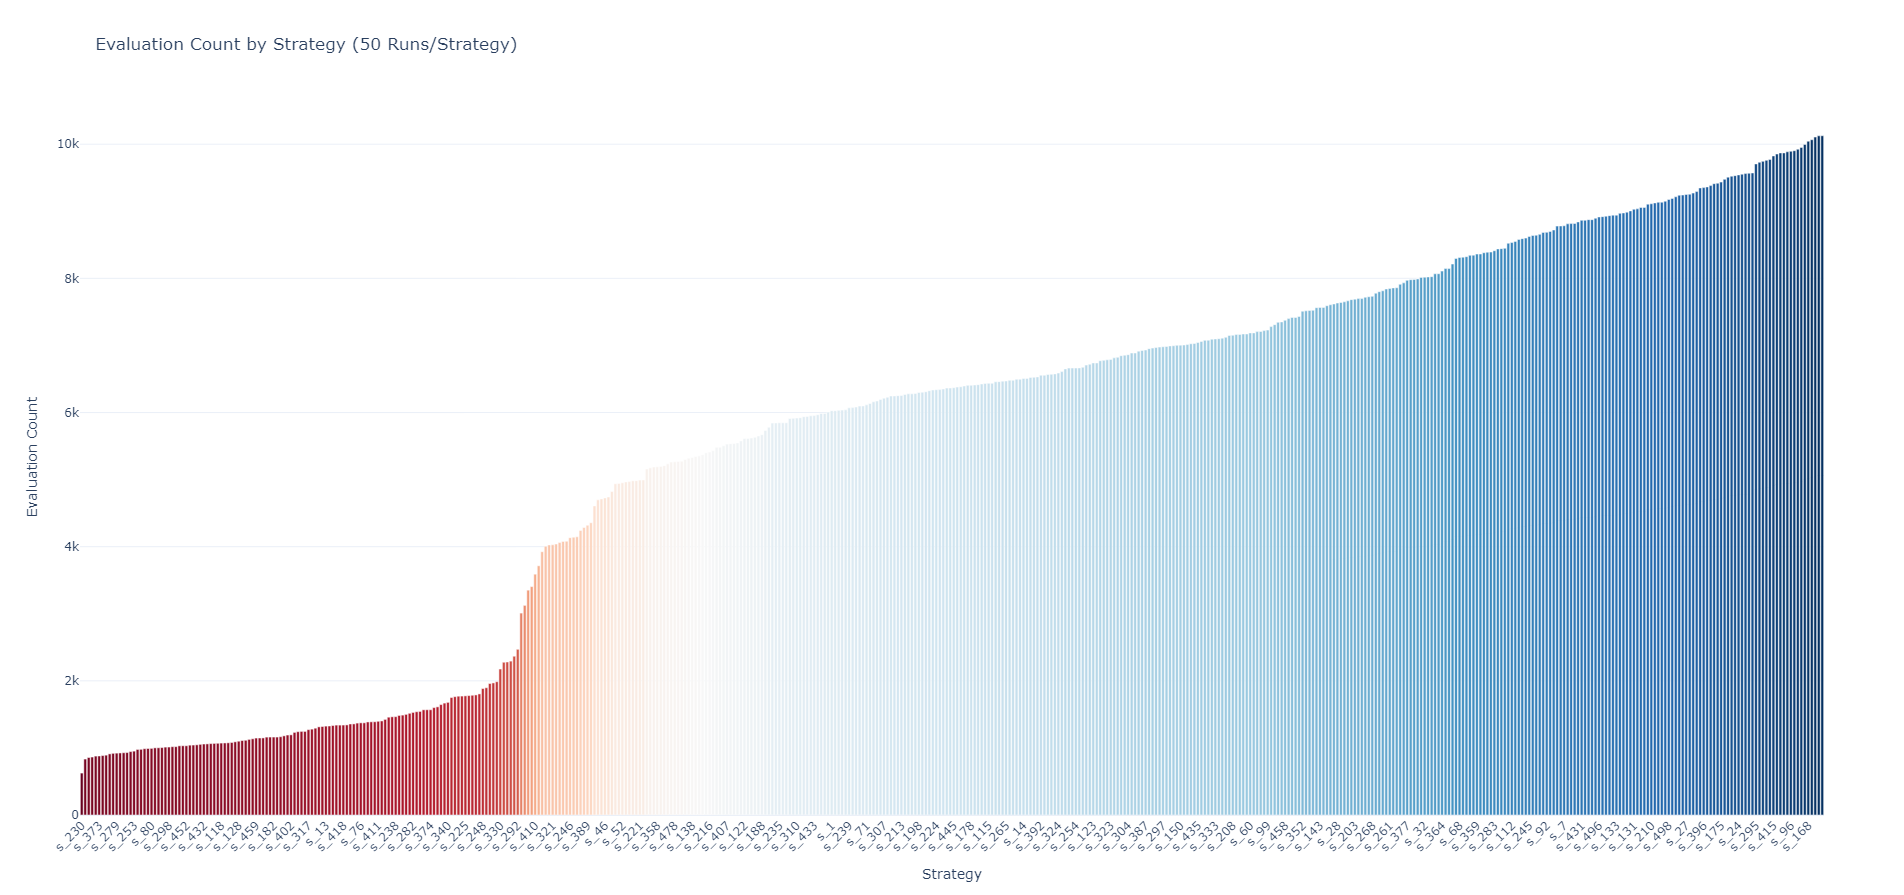
\includegraphics[width=1.2\textwidth]{img/50x500 new.png}}}
    \caption{Plot of the different setups generated, with randomized strategies and parameters}
\end{figure}
\\
The plot above generated shows how the different setups compare to each other, in order to not make a huge list below setup\_38 has been extracted, which was the top performing one:
\\
\begin{verbatim}
    s_38 = {
            'GENOME_SIZE': 8,
            'POPULATION_SIZE': 200,
            'NUM_OFFSPRING_RATE': 0.4,
            'TOURNAMENT_GROUP_SIZE': 0.45,
            'MAX_FITNESS_EVALUATIONS': 10000,
            'fitness_strategy': 'conflict_based',
            'termination_strategy': 'evaluation_count',
            'visualization_strategy': 'terminal',
            'metric_strategy': 'avg_similarity',
            'logging_strategy': 'logger',
            'print_type': 'csv_file',
            'POPULATION_SIZE': 189,
            'NUM_OFFSPRING_RATE': 0.423,
            'RECOMBINATION_RATE': 0.741,
            'MUTATION_RATE': 0.079,
            'TOURNAMENT_GROUP_SIZE': 0.364,
            'initialization_strategy': 'random',
            'parent_selection_strategy': 'tournament',
            'recombination_strategy': 'pmx_dp_rm',
            'mutation_strategy': 'duplicate_replacement',
            'survival_selection_strategy': 'prob_survival',
        }
\end{verbatim}
The problem with analysing the strategies and parameters like this, is that we aren't isolating them everything gets randomized and put into a setup.
\\\\
Below is a plot of some setup, the parameters and strategies for this one are irrelevant; With a genome size of 7 were we are comparing the algorithm with and without genocide
\begin{figure}[ht]
\centering
\makebox[\linewidth]{%
  \setlength\fboxsep{1pt}%<- optional for padding
  \colorbox{black}{%
    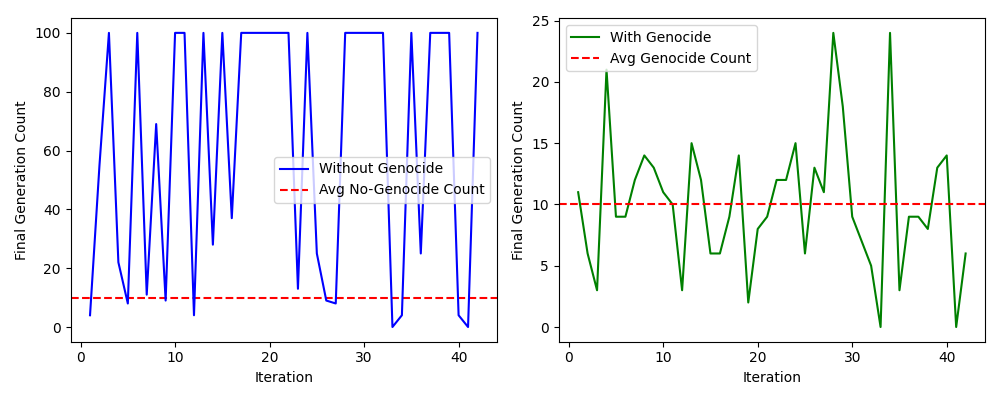
\includegraphics[width=1.2\textwidth]{img/Genome size 7, With and without genocide.png}}}
    \caption{Genome size 7, without and with genocide}
\end{figure}
\\\\
As you can see running the algorithm with genocide provides a higher average.

\section{Results}


\section{Conclusion}
\subsection{Recap}
The N-Queens problem is a well known combinatorial problem, a problem in which the aim is to place N number of queens on a N times N board in such a way that none are attacking each other. This is a very well documented problem \& provided a great way for experimenting and implementing different evolutionary computing algorithms.
\\\\
We started off with some simple code we found in the course material. We began off by modularizing the code in order to easily add and change the different strategies used, we for instance tested different recombinatorial, mutation \& initialization strategies. We also worked with parameter tuning in changing the population sizes, max evaluations count, mutation \& recombination rates. Towards the end we started experimenting with both static and dynamic genocide.
\subsection{Reflections on results}
\subsubsection{Strategies \& parameter tuning}
As mentioned in the \textbf{\textit{5. Results \& Analysis}} finding the most optimal strategies was easier than the parameters, we had clearer answers and the patterns were easier to analyze. We found the most optimal setup to be:
\begin{verbatim}
    optimal_setup = {   'GENOME_SIZE': 8,
                        'POPULATION_SIZE': 116, 
                        'MAX_FITNESS_EVALUATIONS': 10000,
                        'NUM_OFFSPRING_RATE': 0.543, 
                        'RECOMBINATION_RATE': 0.716, 
                        'MUTATION_RATE': 0.065, 
                        'TOURNAMENT_GROUP_SIZE': 0.515, 
                        'MAX_STAGNANT_GENERATIONS': 3,
                        'TOLERANCE': 1e-2,
                        'GENOCIDE_PERC': 0.3,
                        'initialization_strategy': 'random', 
                        'parent_selection_strategy': 'tournament', 
                        'fitness_strategy':           'conflict_based',
                        'recombination_strategy': 'pmx_dp_rm', 
                        'mutation_strategy': 'duplicate_replacement', 
                        'survival_selection_strategy': 'prob_survival',
                        'termination_strategy': 'evaluation_count',
                        'visualization_strategy': 'terminal',
                    }
\end{verbatim}
You can find a more in depth explanation \& analysis of the different parameters \& strategies in the
\textbf{\textit{5. Results \& Analysis}} part. However using the above settings we are able to fast \& consistently find a solution for the N-Queens problem in the least amount of evaluations possible. Whilst bench-marking the different strategies \& parameters against each other we defined one setup being better than the other by the amount of evaluations it took on average to find a solution, the lower the better.
\subsection{Tips on continuing}
While our results demonstrate an efficient setup for solving the N-Queens problem, there is room for improvement, especially in the areas of scalability and parameter tuning. Below, we outline some key areas for further exploration
\subsubsection{Parameter tuning}
A Deeper exploration of the parameters, as mentioned above we worked with for instance tweaking the mutation, population size, max evaluations and more. However this could be expanded upon by running larger tests for in theory better results. The patterns generated by the parameters may be to complex to analyze in two dimensions, this is something one could look into as well. One could use tools like grid search or Bayesian optimization to find parameters \& tools to examine the higher dimensions like PCA (Principal Component Analysis)
\subsubsection{Scalability analysis}
More investigation into how the algorithm scales with extreme sizes of N, it is known that genetic algorithms for this problem out-class backtracking algorithms for larger sizes of N, however testing and tweaking the different strategies for extremer sizes of N might be interesting
\subsubsection{Threading, parallelism \& optimizations}
We did use threading in combination with our parameter tuning to speed the entire process up, however if one where want to for instance explore the point mentioned above experimenting with distributed computing approaches will probably be needed, or simply as a challenge to find a solution as fast as possible
\subsection{Closing Thoughts}
This study and report have demonstrated the effectiveness of evolutionary algorithms both generally and for this problem specifically. It has opened up opportunities for further exploration in areas like parameter tuning, scalability and parallelism. The algorithm can likely be fine tuned in these areas to handle even larger instances efficiently, continuing to outperform traditional methods like back-tracking in time.

\bibliographystyle{ieeetr}
\bibliography{references}

\end{document}
